% Anonymous layout fixture, NOT a dissertation or scientific evidence.
\documentclass[draft]{pnunanomech}
\PNUsetup{
 title-ko={나노메카트로닉스공학과의 국문 박사학위논문 작성 양식 및 자동 참조 검증을 위한 예시},
 title-en={An Example for Verifying the Korean Doctoral Thesis Layout and Automatic Cross-References in Nanomechatronics Engineering},
 author-ko={예시 저자},author-en={Example Author},
 draft-label={서식 검증용 예시 — 실제 학위논문 아님},approved=false
}
\newcommand{\ExampleKo}{이 문서는 연구결과가 아니라 서식 검증을 위한 익명 예시이다. 국문 제목과 영문 제목, 학과명 및 각 구성요소의 위치를 확인한다. 문서의 내용을 추가하거나 삭제한 뒤에도 장절 번호와 표목차, 그림목차 및 참고문헌 번호가 연결되는지 검사한다. 미확정 학위종별과 심사일은 임의로 입력하지 않는다. 본문의 줄바꿈과 문단 배치가 바뀌더라도 글자가 누락되거나 페이지 경계를 벗어나지 않아야 한다.}
\newcommand{\ExampleEn}{This document is an anonymous typesetting fixture, not a report of research findings. It tests the placement of the title, author, affiliation, and abstract heading. It also checks automatic numbering, references, page transitions, and text wrapping. Unconfirmed degree names and examination dates remain blank. The example must never be submitted as a completed dissertation.}
\begin{document}
\PNUMakeCover
\PNUMakeBlank
\PNUMakeApproval
\PNUMakeLists
\PNUAbstract{ko}{\ExampleKo\par\ExampleKo\par\ExampleKo\par\ExampleKo\par 주요어: 서식 검증, 학위논문, 상호참조}
\PNUStartBody
\chapter{서론}\label{chap:intro}
\section{인용과 상호참조 시험}
첫 등장 문헌은 \citep{cioli2022}이다. 다음 문헌은 \citep{salonitis2016}이며, 두 문헌을 함께 참조한다\citep{salonitis2016,cioli2022}. 이 문장은 문헌 내용에 관한 학술적 주장을 하지 않고 인용순서만 시험한다.
\ExampleKo
\begin{table}[htbp]
\centering
\caption{편집 가능한 예시 표}\label{tab:example}
\begin{tabularx}{\textwidth}{lXX}
\toprule 항목 & 검증 내용 & 수용 기준 \\ \midrule
학과명 & 나노메카트로닉스공학과 & 공식 영문 명칭과 대응 \\
페이지 & 앞부분과 본문 구분 & 로마숫자 및 아라비아숫자 \\
참조 & 표·그림·수식 연결 & 번호와 쪽수가 갱신됨 \\
\bottomrule
\end{tabularx}
\end{table}
\begin{figure}[htbp]
\centering
\begin{tikzpicture}[node distance=10mm,every node/.style={draw,align=center,minimum width=35mm,minimum height=13mm}]
\node (a){입력 원고};\node[right=of a](b){LaTeX 조판};\node[right=of b](c){PDF 검수};
\draw[->](a)--(b);\draw[->](b)--(c);
\end{tikzpicture}
\par\smallskip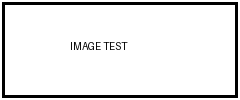
\includegraphics[width=20mm]{tests/image-fixture.png}
\caption{익명 문서 제작 절차 예시}\label{fig:example}
\end{figure}
표~\ref{tab:example}(\pageref{tab:example}쪽), 그림~\ref{fig:example}(\pageref{fig:example}쪽), 식~\eqref{eq:example}의 연결을 확인한다.
\begin{equation}\label{eq:example} y=ax+b \end{equation}
\foreach \n in {1,...,8}{
 \section{장절 및 목차 검증 항목 \n}
 \ExampleKo\par
 \subsection{문단과 특수기호 검증}
 한글 및 영문 ABC, 수학기호 $\alpha,\beta,\Delta,\pm,\times,\leq,\geq,\mu$m의 출력을 확인한다.\par\ExampleKo
 \subsection{쪽번호와 연결 검증}
 \ExampleKo
}
\chapter{검증 정리}
\ExampleKo
\PNUBibliography{references}
\PNUAppendix
\chapter{시험 범위}
이 부록은 선택적 부록의 위치를 확인한다. 본문에 실제로 존재하지 않는 장이나 연구결과를 목차에 만들지 않는다.
\PNUAbstract{en}{\ExampleEn\par\ExampleEn\par\ExampleEn\par\ExampleEn\par Keywords: typesetting; thesis template; cross-reference}
\end{document}
